Consider a neural network with a large number of hidden units relative to the input layer's size.
Such a network is a powerful machine learning system, yet, without regularization, it is prone to overfitting.
Neurons fron a layer can develop dependencies to neurons from the previous layers.
In order to prevent such a thing, we randomly shutdown or ``drop'' neurons by setting their outputs to 0.
This penalizes neurons co-dependencies and allows the net to yields higher results.
Let's explore how we determine whether a neuron should be ``dropped'', and how it affects the forward and backward passes.


\begin{figure}[!ht]
    \centering
    {{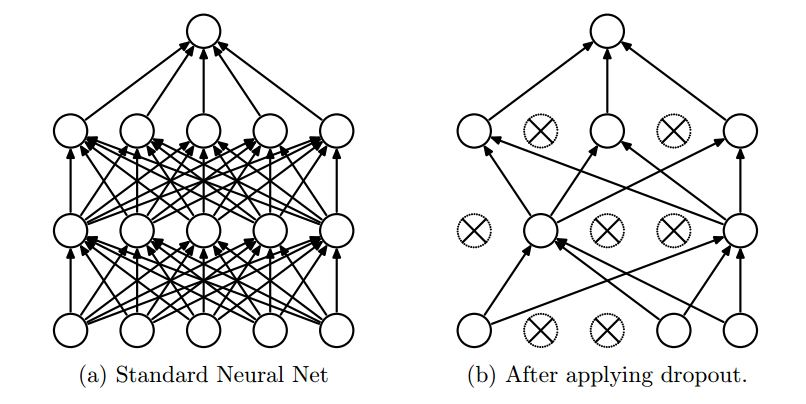
\includegraphics[scale = 0.50]{src/diagrams/dropout.png}}}  
\end{figure}

\begin{itemize}[topsep=-10pt]
\item \textbf{Forward pass}: dropout($o_i$) = $o_i$ with probability p, otherwise 0.
  
During the forward pass we are modifying the network itself,
neurons are randomly dropped from the network such that each neuron can be dropped with probability $p$,
or kept with probability $q = 1- p$.
To do so, for each neuron, we simulate a draw from a Bernoulli distribution by drawing a sample $x$ from a uniform distribution
and dropping a neuron if $x < p$.

We only use dropout when training a net and as such, during training, a neuron's expected input will be scaled down by $q$ such that $o_i = q\sum_{i=1}^K x_i$, where $x_i$ is the neuron's $i^{th}$ input.
Thus, during testing, a neuron will be overloaded as the sum of its inputs will be unexpectedly large.
A solution to this problem could be to scale activation outputs by the keep rate $q$ at test time..
Yet, in the spirit of simplification,
we can instead scale activation outputs by the inverse keep rate $\frac{1}{q}$ during the training phase.


\item \textbf{Backward pass}: $\frac{\partial dropout(o_i)}{\partial o_i} = 0 $ if neuron $i$ is dropped, otherwise 1.

  At a high level, the backward pass is only concerned with computing the partial differential of the forward pass' loss with respect to the
  learnable parameters, namely: the weights and bias of each neuron.
  Yet, at a lower level, we need to compute differentials such as the one described in the equation above as they will be needed
  by previous layers.

  Neurons that have been dropped during the forward pass did not contribute to the scores and consequently to the loss of the net.
  Thus, their partial derivatives are zeroed, so that their weights will not be wrongly updated at the end of the backward pass.
\end{itemize}



